\section{Overview}

\subsection{Original Design and Performance}

The CLAS Cherenkov detector~\cite{Adams:2001kk} was instrumental in identifying electrons in the CLAS
spectrometer in Hall B during the Jefferson Lab 6~GeV era. It was used to provide electron/pion discrimination
with an efficiency $> 90\%$.

The system consisted of identical detectors in each of the six sectors on the CLAS Forward Carriage, each
containing:

\begin{itemize}
	\item 108 lightweight adjustable mirrors
	\item 36 Winston light collecting cones
	\item 36 5-in Photonis X4500B PMTs
	\item 36 magnetic shields
	\item C$_4$F$_{10}$ gas, index of refraction: 1.00134
\end{itemize}

The optics of each module was designed to focus the Cherenkov light onto a photomultiplier tube (PMT) associated
with that module and located in the region obscured by the CLAS torus magnet coils. Figure~\ref{fig:optics} shows
the optical arrangement of one module. The array of the modules in one sector is shown in \F{ltccArray}.

\begin{figure}[ht]
	\centering
	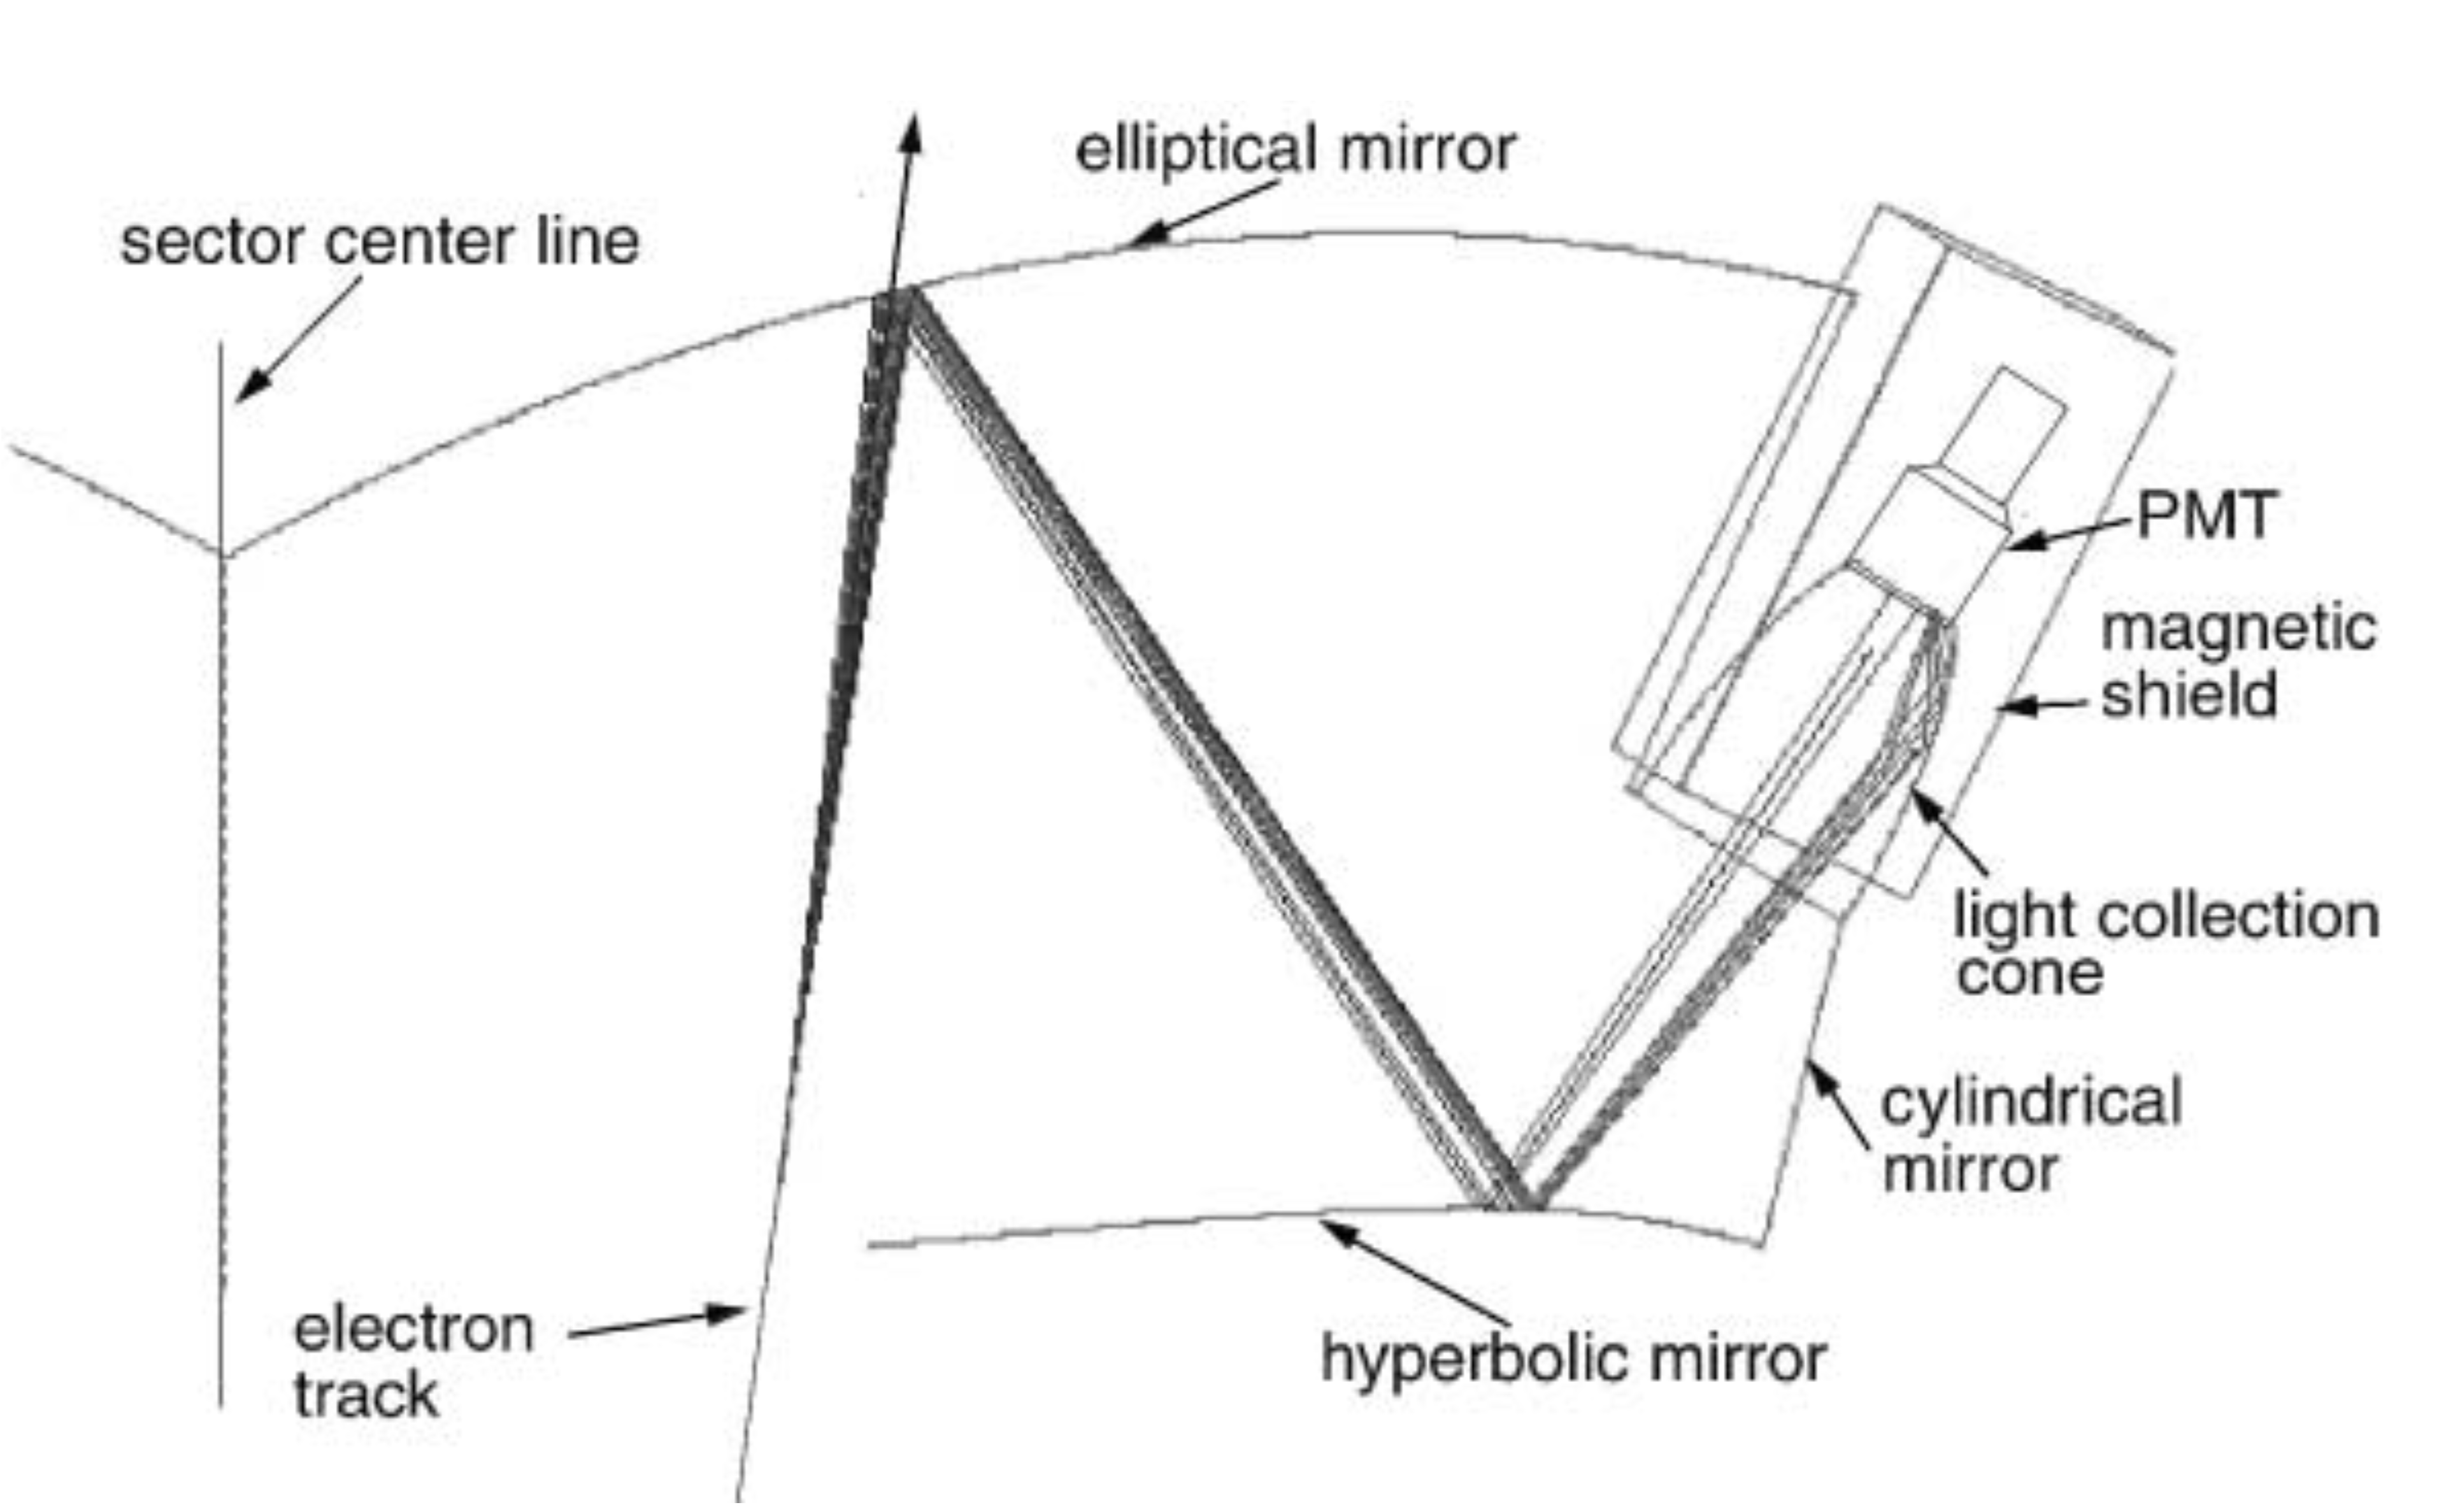
\includegraphics[width=1.0\columnwidth,keepaspectratio]{img/optics.png}
	\caption{Arrangement of one of the 216 modules of the CLAS Cherenkov detector, showing the optical and
          light collection components.}
	\label{fig:optics}
\end{figure}

\begin{figure}[ht]
	\centering
	\includegraphics[width=1.0\columnwidth,keepaspectratio]{img/ltccArray.png}
	\caption{A schematic diagram of the array of optical modules in one of the six Cherenkov detectors, highlighting
          the main system components.}
	\label{fig:ltccArray}
\end{figure}

The detector was operational for about 17~years. The typical number of photoelectrons detected for an electron
passing through the detector volume was between 10 and 20. The PMT gain needed x10 multiplier electronics to be
digitized by the readout ADCs and TDCs. The detector had a few malfunctions: it had significant gas leaks, the
mirror alignment had inefficiencies that reduced the signal strength, and the mirror supports were broken in all
sectors, affecting the optics and system efficiency.

\subsection{Detector Upgrade}

With the 12~GeV energy upgraded accelerator~\cite{TDR12}, the momentum of the particles in Hall~B increases
substantially. Given the pion Cherenkov threshold of 2.6~GeV, the detector cannot provide a good electron/pion
discrimination for most energies and a new High Threshold Cherenkov Counter (HTCC)~\cite{htcc-nim} with a
CO$_2$ gas system has been built to provide electron discrimination up to momenta of 6~GeV.

\begin{figure}[h]
	\centering
	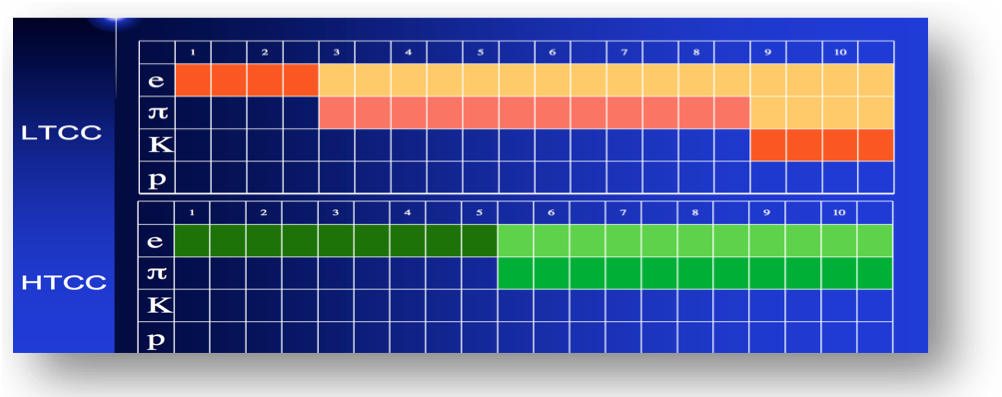
\includegraphics[width=0.99\columnwidth,keepaspectratio]{img/newScope.png}
	\caption{The momentum coverage of the refurbished LTCC to provide for charged pion/kaon discrimination.
          The top row indicates the particle momenta in GeV. The gray boxes indicate the range for which particles
          produce a signal in the LTCC. The pion/kaon discrimination is provided from about 3.7 to 8.5~GeV.}
	\label{fig:newScope}
\end{figure}

The heavier C$_4$F$_{10}$ gas can still be used to discriminate pions from kaons (see \F{newScope}), thus the
detector was refurbished to a Low Threshold Cherenkov Counter (LTCC). The individual detector boxes have
been modified to:

\begin{itemize}
	\item Support the new scope of pion/kaon discrimination;
	\item Address the gas leaks and other hardware inefficiencies.
\end{itemize}
